\documentclass[10pt,twocolumn]{witseiepaper}

% All KJN's macros and goodies (some shameless borrowing from SPL)

\usepackage{KJN}
\usepackage{amsmath,amsfonts}
\usepackage{listings} 
\usepackage{tikz}
\usepackage{verbatim}
\usetikzlibrary{shapes.arrows}
\usetikzlibrary{shapes.geometric}
\usetikzlibrary{plotmarks}
\usetikzlibrary{matrix}
\usepackage{pgfplots}
\usepackage{circuitikz}
\usepackage{pdfpages}
\usepackage{placeins}
\usepackage{dblfloatfix}
\usepackage{graphicx}
\usepackage{caption}
\usepackage{subcaption}
\usepackage{url}
\makeatletter
\g@addto@macro{\UrlBreaks}{\UrlOrds}
\makeatother
\usepackage{cleveref}
\usepackage{color,soul}
\usepackage{float}

\pagestyle{plain}

\addtolength{\oddsidemargin}{-.15in}
\addtolength{\evensidemargin}{-.15in}
\addtolength{\textwidth}{0.5in}

%%%%%%%%%%%%%%%%%%%%%%%%%%%%%%%%%%%%%%%%%%%%%%%%%%%
\begin{document}
	
	
\title{ELEN4012 PROJECT PLAN - }
	
\author{Jared Ping (704447) \& Lara Timm (704157)
	\thanks{School of Electrical \& Information Engineering, University of the
			Witwatersrand, Private Bag 3, 2050, Johannesburg, South Africa}
}
	
%%%%%%%%%%%%%%%%%%%%%%%%%%%%%%%%%%%%%%%%%%%%%%%%%%%
\abstract{This report outlines a project plan to implement an Internet of Things (IoT) based smart parking system to alert drivers of available parking bays. The project plan uses Arduino nano and ESP-8266 development boards, ultrasonic sensors, Radio Frequency (RF) communication, the ThingSpeak cloud IoT platform and the Android framework in an attempt to give the project the best chance of success. Testing methodologies have been outlined to quantify the successful operation of the system. Research into IoT hardware, communication technologies, deployment methodologies, data management and data presentation is conducted and analysed. By considering all possible design configurations and flaws that could be encountered, an appropriate and efficient project design is proposed. The project, from design to demonstration, should take 6 weeks.}
	
\keywords{Android, Arduino, ESP-8266, Internet of Things, RESTful API, ThingSpeak, Wireless Sensor Network}
	
\maketitle
%%%%%%%%%%%%%%%%%%%%%%%%%%%%%%%%%%%%%%%%%%%%%%%%%%%%
\section{INTRODUCTION}

% GOOD PAPER FOR GENERAL SHIT - https://www.researchgate.net/profile/Carlo_Guarnieri_Calo_Carducci/publication/282855975_Design_of_a_Low_Cost_Multipurpose_Wireless_Sensor_Network/links/579e07e308ae6a2882f53965.pdf


The digital age has seen a massive increase in the interest in digitizing all aspects of life. The Internet of Things (IoT) is large range of systems, described by the International Telecommunication Union (ITU) as "a global infrastructure for the Information Society", which make use of information and communication technologies to interconnect things~\cite{wortmann_internet_2015}. An IoT-based parking monitoring system aims to allow parking availability tracking in real time via a mobile application, building towards transforming the University of the Witwatersrand into a  Smart Campus. Contained within the remainder of this report is a project plan to design, construct and test a Smart Parking system.

\vspace{1em}
\section{BACKGROUND AND CONTEXTUALISATION}
	The purpose of this section is to demonstrate techniques to identify and communicate parking bay availability. This process includes data acquisition and processing using a sensor module, the deployment of the sensor module, wireless data communication, data management and data presentation. For a minimum viable product, each sensor module must consist of a sensor, microcontroller (MCU), communication module and power supply.

	\subsection{Hardware Choices} 
	
		The available and preferred hardware options for the sensor module are considered in the sections that follow.
	
		\subsubsection{Microcontroller} $   $
		
			When choosing an MCU for an IoT system it is important to consider a number of factors. These include the MCU's power consumption, number and availability of I/O ports, how the MCU will interface with the sensors and how the sensor modules will communicate with one another. Additional considerations are the ease of use of the MCU as well as its the size and expense.
			
			A popular, versatile and relatively inexpensive MCU platform is the Arduino Platform. Owing to their small size and reasonable price, the \textit{Arduino Nano V3} and \textit{Arduino Pro Mini} development boards are considered. Arduino devices are well documented with a wide array of libraries, provided through extensive community support, which support a range of inexpensive sensor and communication modules. The \textit{Nano} is advantageous over the \textit{Pro Mini} due to its ease of programming, greater availability and lower current draw during normal operation. Greater power consumption in the \textit{Pro Mini} occurs due to an inefficient on-board power regulator integrated circuit (IC).

			An alternative to the Arduino platform is the ESP8266-based development board range. 
			These boards are designed to cater for low consumption requirements, such as the bare-bones ESP8266 MCU, through to intensive processing requirements, such as the dual core ESP32 MCU. The development boards come pre-built with a \mbox{Wi-Fi} module, among other communication modules, which negates the need for additional communication hardware~\cite{esp12e}.
			
		\subsubsection{Sensor} $   $
			
			The sensor chosen to detect vehicle presence in an open air parking lot should be tolerant of the environmental conditions in which it must operate. The sensor module will be exposed to large amounts of ambient light, varying light conditions, fluctuating temperatures and rain. As such, the chosen sensor should not rely on light to detect vehicles, should not be significantly affected by changing temperatures and should be weatherproof. Considering also that the cost per sensor module should be as low as possible, connecting multiple sensors to a single MCU is a reasonable design choice.
			
			This specification suggests an accurate distance/proximity measurement sensor with a reasonable range (0.5 - 2~m). Examples of such sensors include microwave radar, RFID, passive infrared and ultrasonic sensors~\cite{parkingSystem}. An ultrasonic distance measurement sensor is preferred for this application due to its high accuracy and ability to set a user-defined range.
			
		\subsubsection{Communication} $   $

			The method of communication between the sensor nodes is a key design consideration as many options are available, each with their own benefits and trade-offs. A range of communication modules exist which are compatible with most common MCUs. These include Wi-Fi, RF, Bluetooth and NFC communication standards. The chosen mode of communication should be robust and reliable as to prevent data loss during transmission. Furthermore, the communication modules should be able to endure a range of outdoor weather conditions as well as obstructions which may exist between two modules.

			The solution should be designed to cater for a system that can be easily and efficiently scaled. This requires the abundant availability of channels within the chosen communication scheme to prevent bandwidth throttling within the sensor network. It is pivotal that a power efficient communication scheme is utilised. Power consumption is proportional to transmission range, and a communication module with variable power modes would be ideal for a scalable and power efficient solution. Enabling line of sight between nodes would require less power as transmission does not need to occur through any obstacles.
			
		\subsubsection{Power Supply} $   $
			
			The sensor network should be portable and self-sufficient, requiring a power scheme that is independent. The sensor network requires supply modules which are well regulated and offer large capacity. Additionally, the modules should be renewable and affordable. Rechargeable batteries cater for this exact purpose.

			A range of rechargeable batteries exist which include lithium ion (Li-ion), lithium polymer (Li-Po) and nickel metal hydride (Ni-Mh) options. Li-ion batteries generally offer high capacity in 3.7~V multiples but are known to be quite dangerous when exposed to high temperature ranges~\cite{li-ion}. Li-Po batteries offer a large range of capacities in 3.7~V multiples but the price increases exponentially as capacity increases~\cite{li-po}. Ni-Mh batteries are versatile in offering a large range of capacities as well as a range of voltages~\cite{ni-mh}.

			The chosen supply will need to be regulated to ensure stable operation of the sensor nodes, as any fluctuation in supply may damage or prevent the sensor nodes from functioning correctly. To ensure the supplied voltage is at an expected level, the use of a boost converter could be utilised to step up the default supply voltage of the batteries.
	
	\subsection{Communication Technologies}
	
		The Industrial, Scientific and Medical (ISM) band refers to a group of radio bands that are unlicensed and internationally reserved for the use of RF transmissions. Any communication operating within the ISM band should be tolerant of interference from other ISM equipment. There has been a surge in low-power, short-range communication platforms utilising the ISM band such as Bluetooth, \mbox{Wi-Fi}, NFC and mobile networks~\cite{ism}. Thus a large variety of communication methods are available offering a range of power consumptions, transmission ranges and data rates.
	
		A variety of application-appropriate communication technologies are available to communicate between sensor nodes. These are discussed in the sections that follow.
		
		\subsubsection{Wi-Fi} $   $
		
			This communication scheme is well known and easily accessible for use within the IoT market. It's range will vary depending on a number of factors, including the specific IEEE 802.11 protocol which the module is utilising, the strength of the module's transmitter, and radio interference from the surrounding environment~\cite{802.11}. Low energy consumption modules require between 14~dBm (25~mW) to 19~dBm (79~mW) for typical transmission with a data rate of 72~Mbps~\cite{esp12e}. At maximum transmission power in an open environment, a maximum transmission distance of approximately 100~m is achieved~\cite{esp12e}. The ESP8266 \mbox{Wi-Fi} module allows four simultaneous client connections with unidirectional communication~\cite{esp12e}.

		\subsubsection{Bluetooth} $   $
		
			Bluetooth is another well known communication scheme which is available within the IoT market. Bluetooth utilises the IEEE 802.15.1 standard. Multiple variants exist which offer differing combinations of low energy consumption, high data rates and long transmission distances~\cite{802.15.2}. Low energy consumption modules require a maximum of 3~dBm (2~mW) for a typical transmission, having a maximum range of approximately 150~m and a data rate of 0.23~Mbps~\cite{BLE112}. The long range variant offers a maximum transmission distance of approximately 450~m at a data rate of 0.23~Mbps, and requires 8~dBm (6~mW) to transmit~\cite{BLE112LR}. The number of simultaneous connections allowed varies per device, with the maximum amount being seven, with unidirectional communication~\cite{bluetooth-users}.

		\subsubsection{Radio Frequency} $   $
		
			A range of RF-based transceivers exist which utilise different ISM bands. The NRF24 refers to a protocol used by Nordic Semiconductors which utilises the 2.4~GHz ISM band for RF communication~\cite{nrf24}. Nordic has produced a range of NRF24 based transceivers which have become prominent within the IoT market due to their low cost and adjustable power consumption. The nRF24L01+ transceiver, for example, offers a maximum transmission distance of approximately 100~m with a data rate of 0.25~Mbps and a transmission power requirement of 0~dBm (1~mW)~\cite{nrf24}. Furthermore, the data rate can be configured up to 2~Mbps and transmission power modes can be selected ranging down to -18~dBm (16~$\mu$W)~\cite{nrf24}. These transceivers facilitate 125 simultaneous connections with bidirectional communication~\cite{nrf24}.
			
			An alternative is the RFM69 transceiver, which offers similar operating characteristics to the NRF24-based transceivers but operates in the 433/868/915~Mhz ISM bands and supports up to 255 simultaneous connections~\cite{rfm69}. Naturally, the RFM69 transceiver exhibits marginally higher power requirements to sustain these capabilities and is more expensive than the NRF24-based transceivers~\cite{rfm69}.
	
	\subsection{Deployment Methodologies}
		The parking system is to be deployed in the \textit{3rd, 4th and Postgraduate} parking lot near the Flower Hall building, located on West Campus of Wits University. The designed system covers 72 parking spaces, with four sensors being monitored by each MCU. As such, 18 hardware modules need to be packaged and deployed. \figref{fig:deployment} shows the planned deployment layout. Considerations have been made for the module rigidity, resistance to environmental conditions, security and positioning.
		
		\begin{figure}
			\centering
			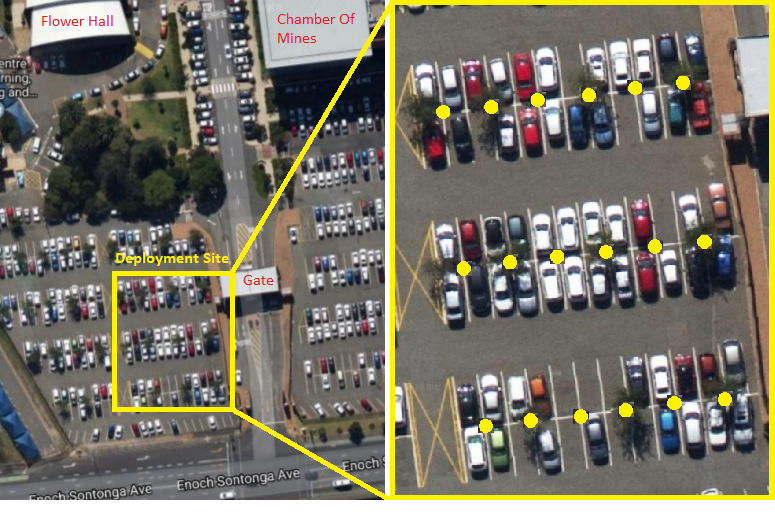
\includegraphics[width=1\columnwidth]{media/deploymentSite.png}
			\caption{Smart Parking deployment site (Google Maps satellite view) and module placement map}
			\raggedright
			\label{fig:deployment}
		\end{figure}
	
		When deployed, the hardware should be raised from ground level, not only to prevent the circuitry from being damaged by excessive water runoff, but also to provide the ultrasonic sensors with the best viewing angle; ensuring that all shapes and sizes of vehicles can be detected. The use of an ultrasonic sensor provides challenges regarding waterproofing, as a result of ultrasonic waves being impermeable to almost all materials. As such, there cannot be any barrier between the sensors and the cars being detected, requiring a runoff system that will keep this circuitry dry. 
		
		Raising the hardware requires that the sensor nodes are resilient to strong winds, and should not break if they are bumped by vehicles driving into or between parking spaces. In an attempt to keep costs to a minimum, a PVC stand is proposed that will be rigid, stable and provide the right topology to detect vehicles at average bumper height. A top and isometric view of the proposed stand is provided in \figref{fig:stand}. Considerations must be made for the security of the modules once they are deployed.
		
		\begin{figure}
			\centering
			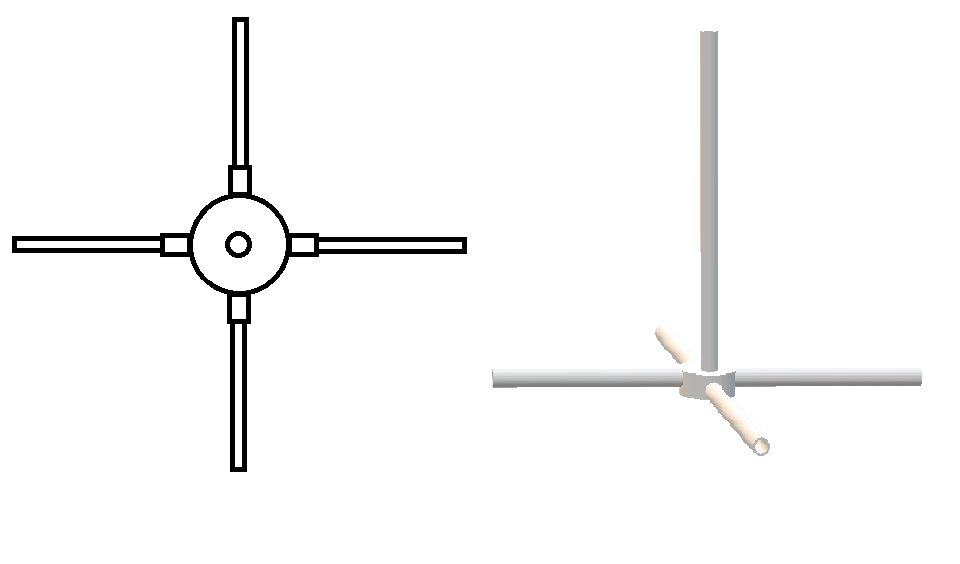
\includegraphics[width=1\columnwidth]{media/topIsoStand.png}
			\caption{Top (left) and isometric (right) view of the proposed PVC stand}
			\raggedright
			\label{fig:stand}
		\end{figure}
	
	\subsection{Data Management}
	
		Optimised collection and processing of sensor data is required to provide the relevant parking bay information to users. These components are described as in the sections that follow.
		
		\subsubsection{Mesh Network} $   $
		
			The concept of a mesh network relates to a network topology in which infrastructure nodes, being the sensor nodes, are connected in a range of configurations to allow for the efficient routing of data between the nodes within the network~\cite{mesh}. In this specific scenario, the goal relates to implementing a network topology whereby all sensor data is successfully transmitted to the gateway node within the network. Furthermore, the mesh network should be designed in a way that facilitates the ability to enable self-configuration of the nodes within the topology. This allows for dynamic distribution of workloads, which is important in the scenario where a node may happen to fail~\cite{mesh}. This results in improved fault-tolerance and minimised system maintenance. The major considerations of the topology design in the context of this project are node transmission distance and node power consumption. Two topologies offer varying combinations of these factors.
			
			\figref{fig:single} illustrates a topology whereby a node will always transmit to its adjacent node until the gateway is reached. This results in a topology which yields a low transmission distance requirement but a high power requirement due to the amount of time which nodes must be powered as well as a large total number of transmissions per round of data gathering. 
			
			\figref{fig:segment} illustrates a topology whereby nodes are bound to segments and within each segment all nodes in a row will transmit to a single node. The receiving nodes will then transmit to the adjacent segment and the receiving node will transmit to the gateway node via the closest row node. This results in a topology which yields a longer transmission distance requirement but a lower power requirement due to the reduced time which nodes must be powered as well as a lower total number of transmissions for per round of data gathering.
			
			\begin{figure}
				\centering
				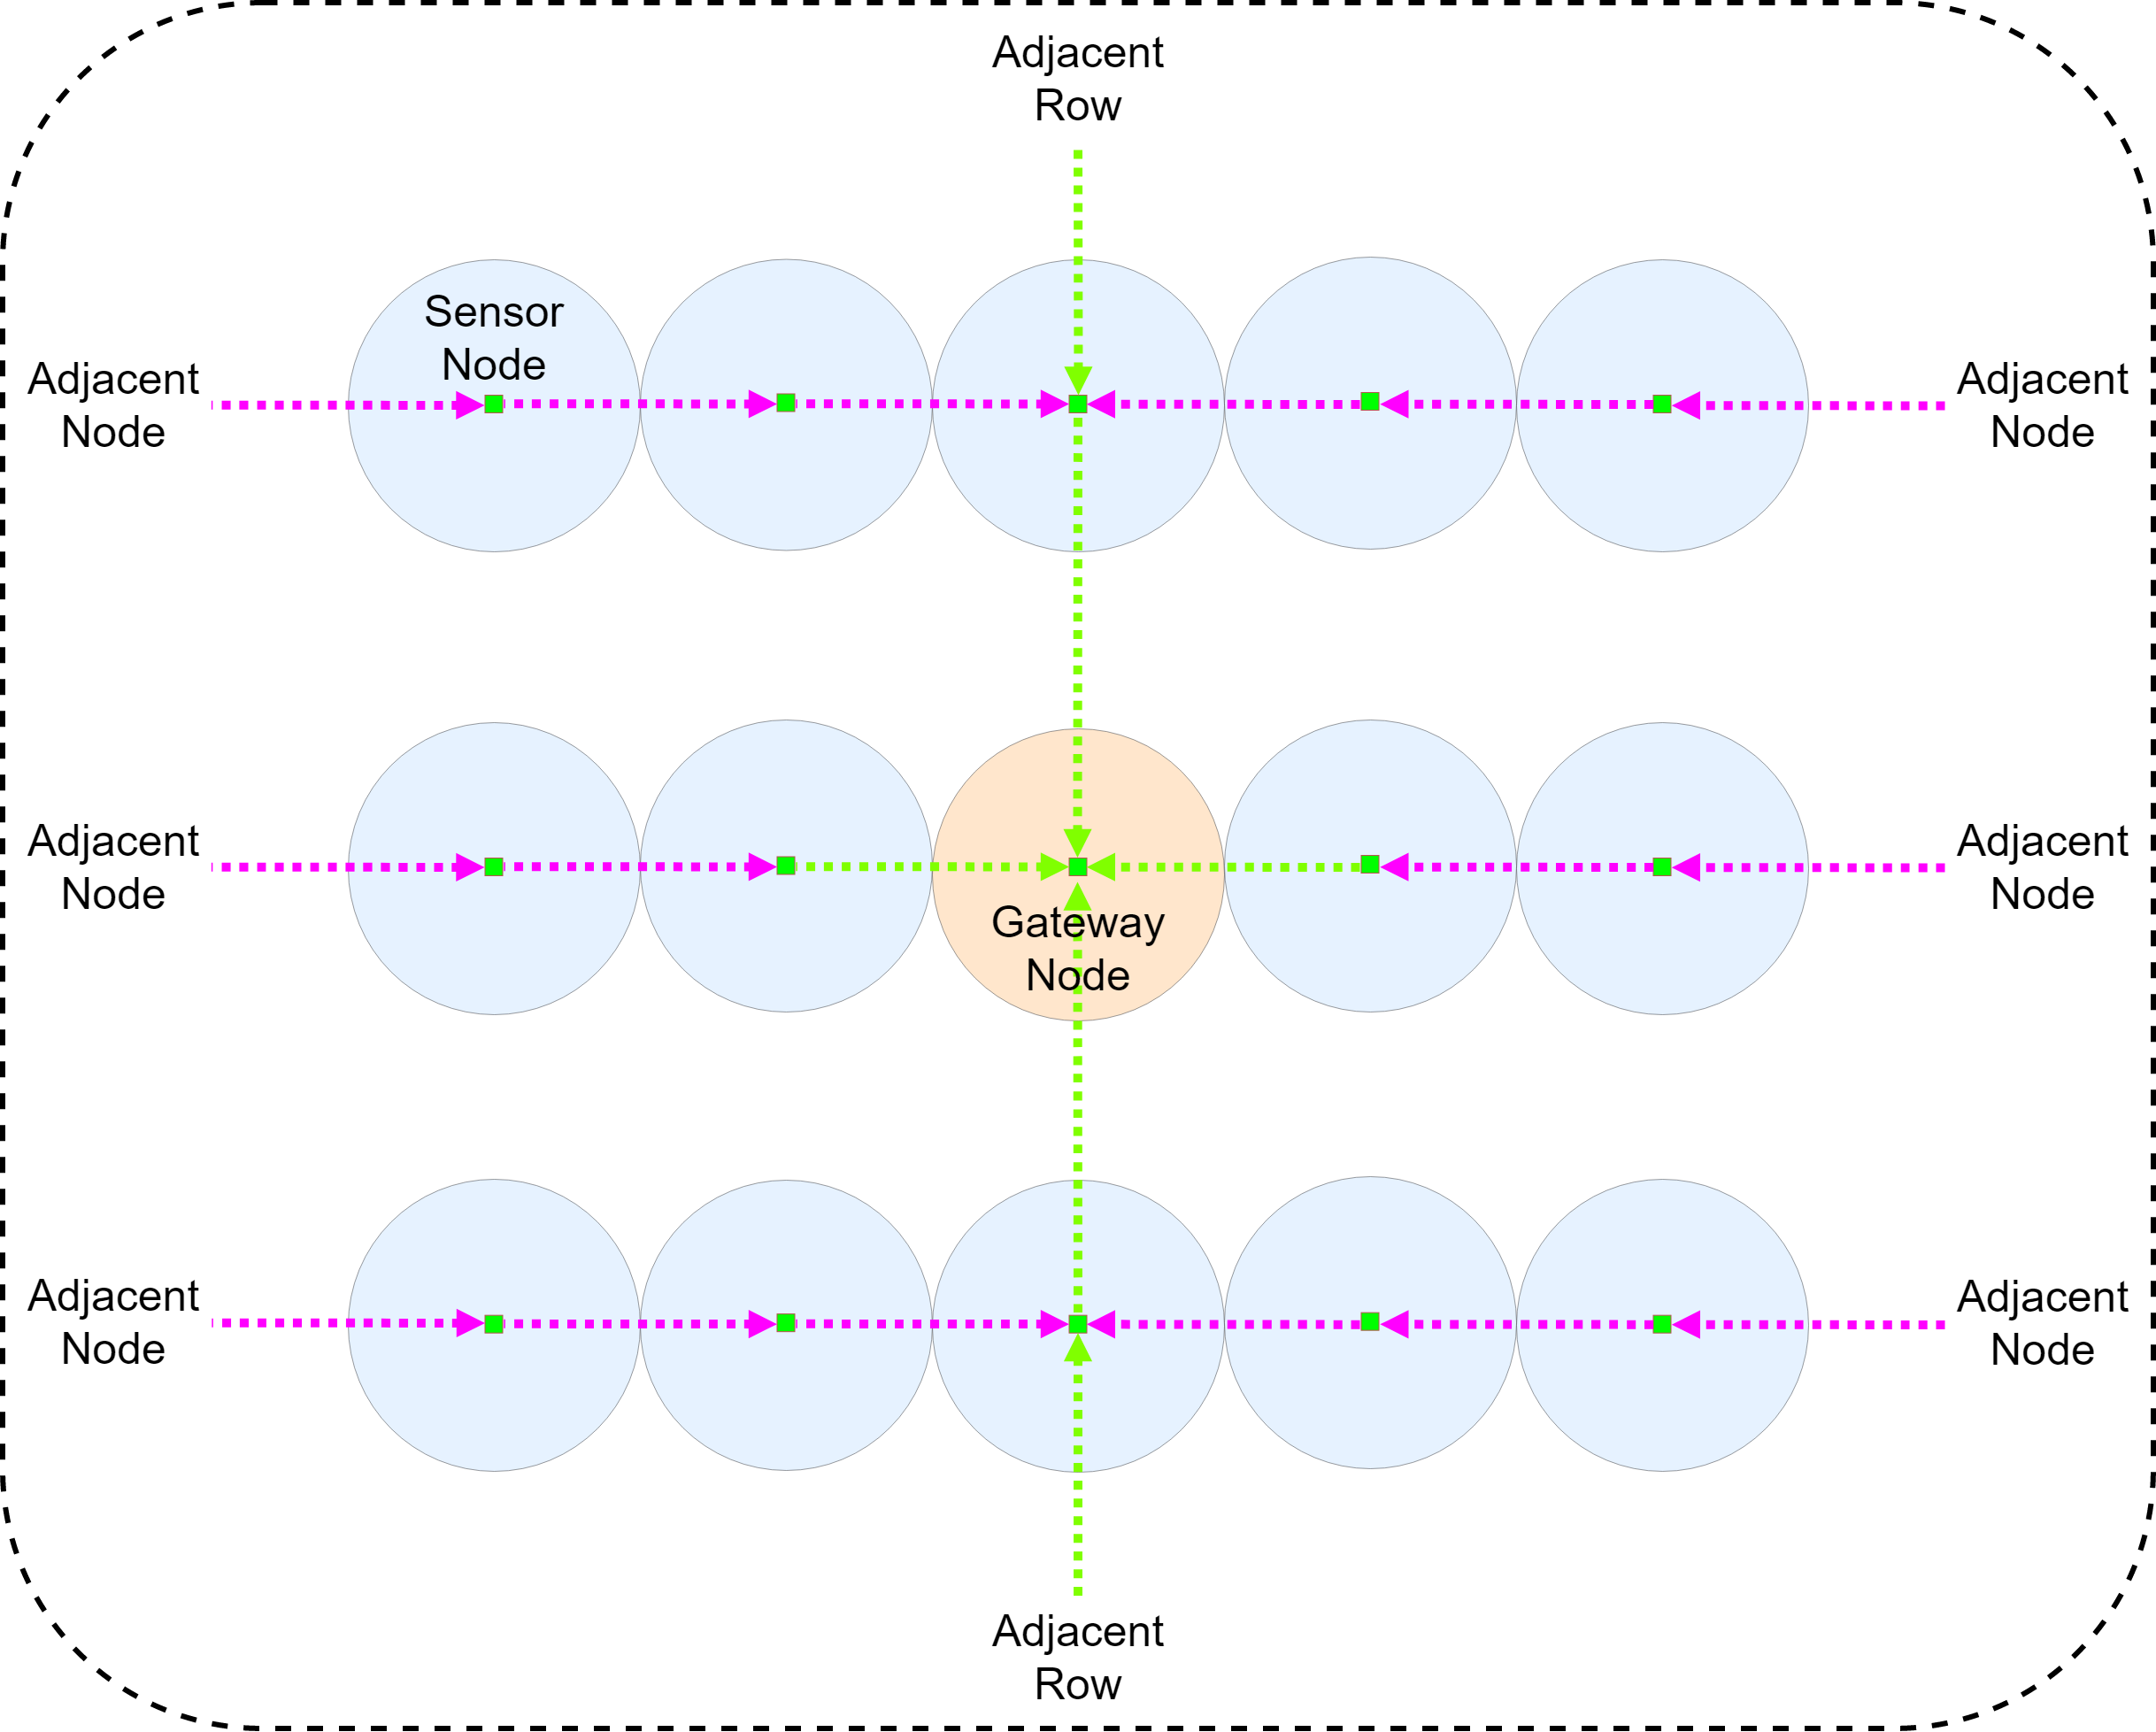
\includegraphics[width=1\columnwidth]{media/hop-mesh.png}
				\vspace{1em}
				\caption{Node mesh network which utilises single node hop communication for short range transmission}
				\raggedright
				\label{fig:single}
			\end{figure}
		
			\begin{figure}
				\centering
				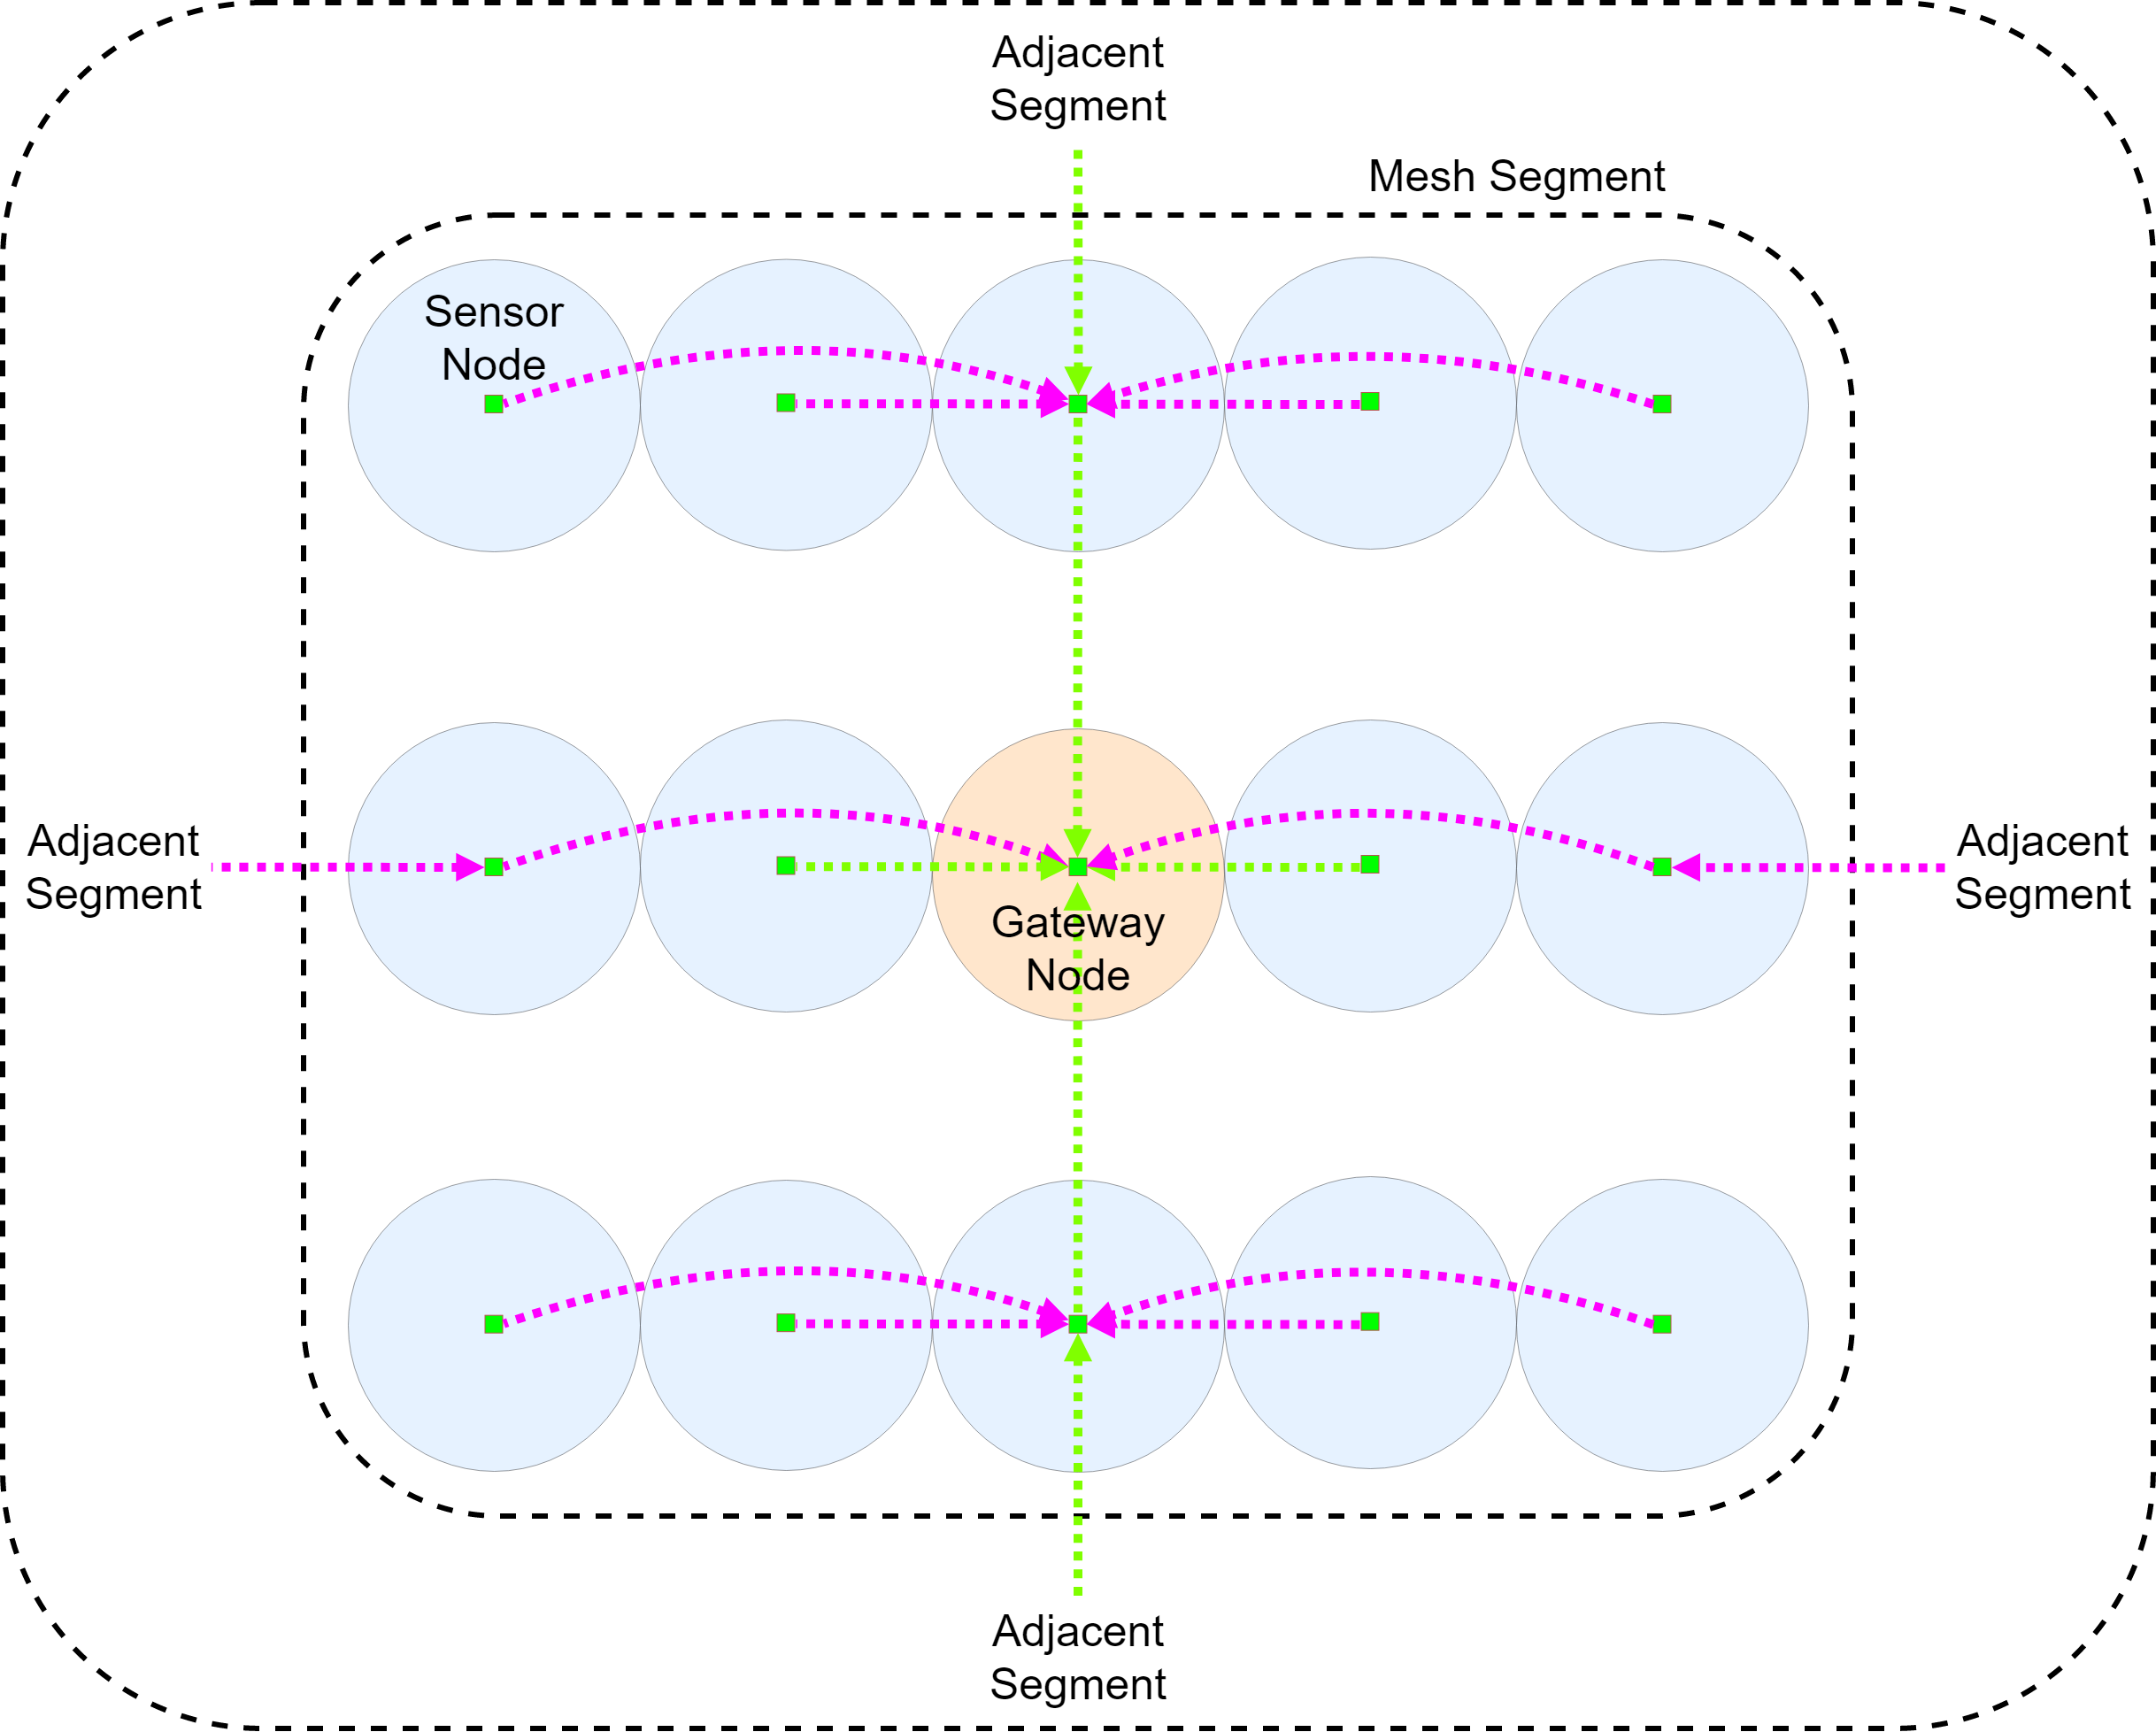
\includegraphics[width=1\columnwidth]{media/segment-mesh.png}
				\vspace{1em}
				\caption{Node mesh network which utilises node-skip communication in a segmented mesh configuration for longer range transmission with fewer hops}
				\raggedright
				\label{fig:segment}
			\end{figure}
	
		\subsubsection{Data Upload} $   $ \label{sec:data_upload}
		
			The following communication methods are considered in uploading sensor data to the utilised data platform.
			
				\textbf{GSM/GPRS:}~~
				Global System for Mobile (GSM) communication, also commonly referred to as 2G, due to being a second-generation cellular network provides support for voice calls, Simple Message System (SMS) and data communication via General Packet Radio Service (GPRS). GPRS is a packet switching technology which can provide idealised data rates between 0.056~Mbps to 0.114~Mbps~\cite{gprs}. To utilise GPRS for data communication, an Access Point Name (APN) and username/passward pair is required from a network operator~\cite{gprs}.
				
				GSM modules are commercially available and are compatible with most major development boards. These modules require a Subscriber Identification Module (SIM) which is an integrated circuit with the purpose of securely storing the International Mobile Subscriber Identity (IMSI) number with its corresponding authentication key~\cite{imsi}. These are used to identify and authenticate subscribers on the mobile network. Such an example of a GSM module is the common Quectel M10 module which is a quad-band GSM/GPRS modem requiring a supply of just 3.4~V~\cite{m10}.

				\textbf{Wits Wi-Fi:}~~
				The University of the Witwatersrand (Wits) offers a high speed network, offering local and international data rates of 10~Gbps and 589~Mbps respectively~\cite{wits-speed}. Due to the constant need for connection on the main campus, the network is extremely reliable with minimal down-time.
				
				The use of a development board such as the ESP12-E, which features a built in Wi-Fi module, could easily be used as a gateway node for the sensor network. This module could periodically collect all respective sensor data and thereafter connect to the Wi-Fi network provided by Wits to upload the sensor data to the chosen data platform~\cite{esp12e}.
			
				\textbf{4G/LTE:}~~
				This is the fourth generation of broadband cellular network technology, succeeding 3G. This generation places emphasis on data rates. This is demonstrated in modules such as the Quectel EC25 Long-Term Evolution (LTE) category 4 module which offers download and upload data rates of up to 150~mbps and 50~mbps respectively, requiring a supply of  5~V~\cite{ec25}. This caters for solutions where large amounts of data needs to be transferred continuously.

		\subsubsection{Data Platform} $   $
		
				\textbf{AWS Greengrass:}~~
				Amazon Web Services (AWS) offers Greengrass which is software that facilitates the running of local compute, messaging, data caching, synchronisation, and machine learning capabilities for connected IoT devices in a secure manner. It provides useful off-line capabilities by still allowing devices to run AWS Lambda functions, synchronise device data, and communicate with other devices~\cite{greengrass}. Greengrass is network optimised, ensuring the cost of transmitting data to the cloud is kept to a minimum~\cite{greengrass}.
				
				Greengrass extends AWS to IoT devices, allowing them to act on generated data, whilst providing the cloud platform for management, analytics, and storage of the device data. ?? (refactor sentence) A range of programming languages and programming models which facilitate the ability to create and test device software in the cloud, followed by deploying it to connected devices~\cite{greengrass}??. 
				Data filtering can be effected so that only key information is extracted and transmitted to the cloud. Greengrass continuously authenticates and encrypts all device data throughout the connection process by utilising the Message Queuing Telemetry Transport (MQTT) protocol~\cite{greengrass}. End-to-end security is effected using asymmetric key authentication over Transport Layer Security (TLS) 1.2~\cite{greengrass}. A maximum of 200 devices are supported per group, and unlimited per an account, with a maximum message size of 128~KB per device transmission to the cloud, and 30 messages being allowed per second~\cite{aws-quota}.
				
				\textbf{Cloud IoT:}~~
				Google Cloud Platform (GCP) offers Cloud IoT which is a fully managed suite of integrated services which facilitate convenient and secure connection, device management and global data collection at a large scale. The collected data can be processed, analysed and visualised in real time and effect any required events as a result. Data is collected by the Cloud IoT Core service which is published to the Cloud Pub/Sub service to provide downstream analytics~\cite{cloud-iot}. Ad-hoc analysis can be performed by utilising the Google BigQuery service~\cite{cloud-iot}. Advanced analytics and machine learning can be performed with the Cloud Machine Learning Engine~\cite{cloud-iot}. Data visualisation can be performed with reports and dashboards in Google Data Studio~\cite{cloud-iot}.
				
				The Cloud IoT suite provides insights into device operational efficiency, device management and firmware updates. Out-of-box support is provided for leading manufacturers such as Microchip and Arm. Global device management is efficiently managed using Cloud IoT Core's protocol bridge with automatic load balancing and horizontal scaling~\cite{cloud-iot}. Both MQTT and Hypertext Protocol (HTTP) protocols are offered to cater for the configuration of device connections to the cloud~\cite{gcp-security}. End-to-end security is effected using asymmetric key authentication over TLS 1.2~\cite{gcp-security}. There is no limit on the maximum number of connected devices, the maximum message size is limited to 256~KB per device transmission and 100 messages transmissions are allowed per second~\cite{gcp-quota}. Maximum download and upload data rates are limited to 5~Mbps per device~\cite{gcp-quota}.
			
				\textbf{ThingSpeak:}~~
				MathWorks offers ThingSpeak which is an IoT analytics platform service which facilities the collection, aggregation, analysis and visualisation of live data streams in the cloud~\cite{thingspeak}. MATLAB code can be executed in ThingSpeak to perform online processing and analysis of data from devices~\cite{thingspeak}. Both MQTT and HTTP protocols are supported by the platform~\cite{thingspeak}. Analytics can be scheduled to be run periodically or in real-time~\cite{thingspeak}. Third-party services such as Twitter and Twilio can be utilised to communicate device events~\cite{thingspeak}. Native support is provided for common embedded hardware prototyping platforms like Arduino, ESP-8266, Particle and Raspberry Pi~\cite{thingspeak}.
				
				A limit exists on the number of simultaneously connected devices depending on the selected pricing tier. There exists maximum message size limit of 3~KB per device transmission~\cite{thing-quota}. The free pricing tier offers a single channel transmission every 15 seconds with a maximum of three gateway devices simultaneously connected~\cite{thing-quota}. The paid tier offers single channel transmission every second with an unlimited number of simultaneously connected devices~\cite{thing-quota}.
				
				\textbf{SigFox:}~~
				An alternative IoT network is offered by Sigfox whereby it facilitates the broadcasting of device data without the requirement of establishing or maintaining the network connection to do so~\cite{sigfox-tech}. This is designed to reduce signal overhead and offer a compact and optimised connection protocol~\cite{sigfox-security}. This is implemented through the use of Ultra Narrow Band (UNB) modulation~\cite{sigfox-tech}. SigFox operates within the 200 KHz public band~\cite{sigfox-tech}. A RESTful API is used to provide the uploaded data to a platform or application of choice~\cite{sigfox-security}.
				
				A SigFox Software Defined Radio (SDR) module is required to interface with the network and can be obtained as development board shields which are compatible with platforms such as Arduino~\cite{sigfox-tech}. The maximum upload and download data rate ranges between 100~bps and 600~bps and incurs a maximum message size limit of 12~B which can be uploaded a maximum of six times per hour~\cite{sigfox-tech}.
	
	\subsection{Data Presentation}
		Parking bay availability is communicated to the user through data presentation.  The components of this process are described as in the sections that follow.
		
		\subsubsection{API} $   $
		
			Parking bay data needs to be accessible from the data platform which has been configured to receive and process the sensor data from the network. This can be securely and easily implemented through the use of an Application Programming Interface (API). Each data platform offers a preconfigured API to access the processed cloud data through HTTP requests. These requests can be sent from any internet application, which is capable of executing the requests, to obtain the processed data and parse it as required to present information on parking bay availability to the user.
		
		\subsubsection{User Application} $   $
		
			Users require an easily accessible network-based application to access the processed data provided by the data platform. This can be provided through a range of web or mobile applications. The adoption of a web application would prove convenient for a developer due to the vast range of web application frameworks that provide out-of-box API integration and a large range of capabilities for creating a well designed user interface/user experience (UI/UX). The adoption of a mobile application provides fewer design components to be customised for the user however, it provides portability which would allow for a user to easily check their mobile device for an empty parking bay as they are about to enter the parking lot.
			

\section{PROJECT DESIGN}
	\subsection{Hardware Choices} \label{hardware_choices}
	%https://www.electronics-tutorials.ws/transistor/tran_4.html - may be useful
	
		For the sensor nodes a combination of hardware choices have been made. The chosen MCU, an Arduino Nano V3, is powered by two rechargeable AA 1,2~V 3800~mAh \mbox{Ni-Mh} batteries in series, boosted to 5~V using a small boost (step-up) converter circuit module. The 5~V supply rail is also responsible for powering the four HCSR04 Ultrasonic Sensors attached to each module. 
		
		The MCU will be responsible not only for deciding when and for how long the sensors should be powered (using a MOSFET transistor as a switch due to it's low voltage drop) but also to trigger their ultrasonic pulse for distance detection via the return echo signal. This will be achieved through the software configuration in an attempt to reduce power consumption and in turn extend the life of each module before a recharge is required.
		
		The final component of each sensor node is the communication module, the NRF24L01+ transceiver. This module, powered by the 3.3~V rail of the Arduino, transmits the sensor data over the mesh network to the access point, where all sensor data is combined and transmitted to the cloud by the gateway node. The central node/access point consists of an ESP-12E module ,powered similarly to that of the Nano modules mentioned above. The proposed circuit design for a typical sensor node is illustrated in \figref{fig:node-circuit}.

		\begin{figure*}[h]
			\centering
			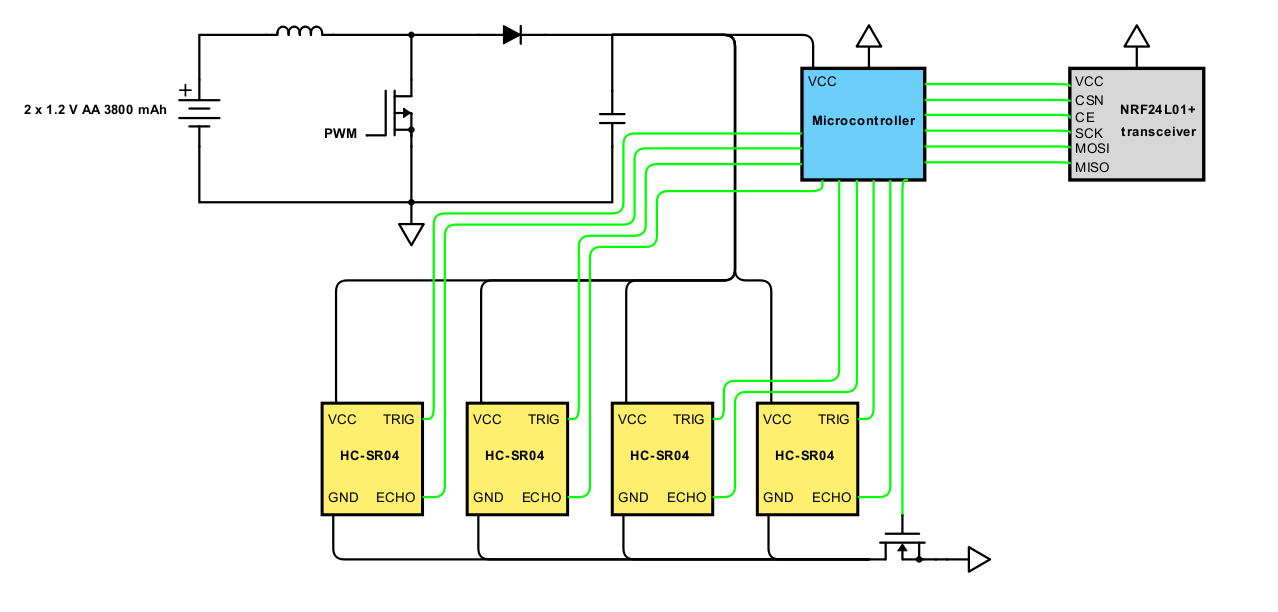
\includegraphics[width=\textwidth]{media/node-circuit.png}
			\caption{Circuit design of sensor node unit containing boost converter, MCU, ultrasonic sensors, and NRF24 transceiver}
			\raggedright
			\label{fig:node-circuit}
		\end{figure*}
	
	\subsection{Communication Technologies}
		The NRF24L01+ transceiver makes use of NRF24 RF technology to transmit data in the free 2.4GHz ISM band. Each transceiver is capable of using 125 different channels in this band~\cite{howToMech_NRF24L01Tutorial}. The module can operate at a range of baud rates, where lower transfer rates increase its range. The achievable range is high but can be decreased with a decrease in transmission amplification power. The modules operate best in open air. To achieve this the devices should be configured such that data is transferred through as few obstacles as possible. 
	
	\subsection{Deployment Methodologies}
	
		The sensor nodes will be deployed in a rigid plastic encasing raised off the ground to average bumper height. This container will have the required windows for the ultrasonic sensors which will need to be recessed from the window. In turn all circuitry will be raised off the bottom of the encasing and drainage holes will be drilled into the underside to enable drainage if water is to enter via the windows.
		
		To raise the casing off the ground, a PVC stand will be assembled from electrical PVC conduits. The base will be held together by a 4 way PVC round box with four balance legs for stability. A vertical pole will be erected from the center of the stand on which the encased sensor module will be attached. The stand will be placed at the junction of four parking spaces and will be weighed down to prevent it from being knocked over.
	
	\subsection{Data Management}
		The design choices made in relation to optimised collection and processing of sensor data are described as in the sections that follow.
	
	\subsubsection{Mesh Network} $   $
	
		The chosen mesh network implements the node-skip topology to reduce the number of node hops required when transmitting sensor data, thus reducing the power consumption of the system. Additional transmitting power will be required for longer distance transmission but is accounted for by optimising the maximum number of nodes which can be skipped.
	
	\subsubsection{Data Upload} $   $
	
		The Wits Wi-Fi network has been chosen as the preferred data upload communication scheme. This is due to the infrastructure being readily available and being highly stable with regards to up-time. The network can be connected to by the gateway node which will be an ESP-12E module with an integrated Wi-Fi module.
		
	\subsubsection{Data Platform} $   $
	
		ThingSpeak will be utilised as the data platform service. This platform is favourable due to its product offerings under a free tier range. Sensor data uploads can be accommodated every 15 seconds which is more than sufficient for the system requirements. A single data upload channel is available which is sufficient due to the system making use of a single gateway node. The maximum message size of 3~KB is sufficient to store all parking bay information. The estimated message size will be 72~B under the assumption that each parking bay is represented by a boolean value. Furthermore, the platform provides native support for the ESP-8266 platform which is to be used as the gateway node.

	\subsection{Data Presentation}
	
		The process of translating raw sensor data into useful information occurs within the data presentation element of the designed solution. This will be served through a mobile application which is to be developed on the Android platform. The application will provide users, being students who wish to search for available parking spots, with a graphical user interface (GUI) in which an aerial view of the surveyed parking bays will be presented. An available parking by will be highlighted in green, whilst an occupied parking bay will be highlighted in red.

		The required sensor data will be obtained from the utilised data platform in the form of a RESTful API which will allow the application to obtain the sensor data through HTTP requests. The updated sensor data will be periodically requested by the application to provide regular GUI updates of available parking bays.
	
\section{PROJECT TESTING}
	A number of system tests are required to validate the design and successful operation of a the IoT parking system. These tests can be categorised and are described in the sections that follow.

	\subsection{Hardware}
		\begin{itemize}
			\item \textbf{System power supply:} The system is sufficiently powered by a suitable power supply that can match the voltage and current requirements of the nodes.
			\vspace{1em}
			\item \textbf{Minimal power consumption:} The physical system should be evaluated to ensure that power consumption is kept to a minimum. This can be achieved through the use of power efficient hardware in conjunction with an optimised software configuration.
			\vspace{1em}
			\item \textbf{System accuracy:} Sensors in the network should provide reliable and accurate readings. The MCUs should process this data to ensure false-positives are mitigated.
			\vspace{1em}
			\item \textbf{Robustness:} The deployed system is able to successfully withstand exposure to a range of environmental conditions. Additionally, the deployed nodes should be resilient to human interference in the form of car bumping or physical tampering.
		\end{itemize}
	
	\subsection{Communication}
		\begin{itemize}
			\item \textbf{Reliable data transfer:} Sensor data should be successfully transmitted between nodes. Additionally, the received data should be error free or errors should be detected and corrected.
			\vspace{1em}
			\item  \textbf{Concurrent connections:} Nodes should be able to successfully receive data from multiple transmitting nodes.
		\end{itemize}
	
	\subsection{Data Management}
		\begin{itemize}
			\item \textbf{Mesh network operation:} Nodes should transmit data towards the gateway node. Transmission will be made to a non-gateway node if the gateway node is more than the maximum allowed number of hops away. Received data should be aggregated and transmitted towards the gateway node until the destination is reached.
			\vspace{1em}
			\item  \textbf{Stable data upload:} The gateway node is able to connect to the Wits Wi-Fi network and periodically transmit the aggregated data of the sensor network to data platform.
			\vspace{1em}
			\item \textbf{Data processing:} Data received from the sensor network is processed in a timely manner and made available through a RESTful API.
		\end{itemize}
	
	\subsection{Data Presentation}
		\begin{itemize}
			\item \textbf{Obtainable data:} Processed data can be requested and retrieved from the data platform via the offered API.
			\vspace{1em}
			\item \textbf{Intuitive GUI:} Application users are able to easily navigate the GUI and understand the presented data to locate available parking bays.
			\vspace{1em}
			\item \textbf{Application updates:} Data updates are periodically requested by the application. Additionally, users can opt to manually request a data update.
		\end{itemize}

\section{PROJECT MANAGEMENT}

	Management of the project includes the management of work, time-management and scheduling. The project can be divided into distinct phases in which specific workflow should take place. \figref{fig:timeline} demonstrates the projected project timeline and the phase progression for the project.
	
	\begin{figure}
		\centering
		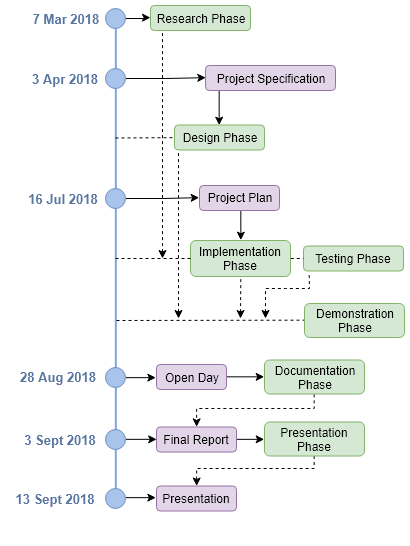
\includegraphics[width=1\columnwidth]{media/timeline.png}
		\caption{Projected timeline of the project, including workflow (green) and deadlines (purple)}
		\raggedright
		\label{fig:timeline}
	\end{figure}
	
	\subsection{Design Phase}
		The design phase consists of a series of iterations of ideation, feasibility analysis, refinement and critical analysis. An important part of the design phase is research, most of which has been presented in the early sections of this report. The final design should ideally be complete before the beginning of the project, yet realistically will continue throughout the implementation and testing phases. 
		
		Both the hardware and software components of the design must be considered here, to the point that all possible design implementations are known and the outcomes can be predicted with reasonable accuracy. 
	
	\subsection{Implementation Phase}
		The implementation phase will start once all hardware components have been procured and the design is finalised. Implementation will begin with the assembly of the sensor nodes as well as their programming. Following this the communication within the mesh network will be set up and tested. Once sensor data can be successfully retrieved by the access point, the data will be transmitted, via the gateway node, to the ThingSpeak cloud. From here a user application will be developed which can retrieve the parking availability data using an available API and presented to the user via an intuitive user interface.
	
	\subsection{Testing Phase}
		Testing will occur throughout the implementation phase. All individual modules, their collaboration, communications and accuracy will be verified as the system is put together. Once the finalised system is deployed into the parking lot, the system success rate will be tested using a statistical approach. Adjustments to improve the system accuracy will be made and, iteratively, a low variance final product will be produced.
		
	\subsection{Demonstration Phase}
		System demonstration is set to take place at Open Day (28th August 2018), six weeks after the beginning of the implementation phase. Preparation for this phase involves creating posters as well as having the system deployed in the parking lot. On Open Day, the developed system will be demonstrated in real time via the mobile application at the group's stand.
	
	\subsection{Documentation Phase}
		The final report is to be written and submitted during this phase. Although documentation will take place throughout all of the previous stages, writing the report is the sole focus of this phase.
	
	\subsection{Presentation Phase}
		The required final presentation is prepared in this phase. It is to be presented to the board of examiners once the final report has been submitted.
	

\section{CONCLUSION}

Research into popular technologies and techniques to develop an IoT based smart parking system has been undertaken. From these, the most plausible options have been chosen, justified and aggregated into a most likely design which will be used to complete the remainder of the project. Essential testing methodologies to validate the system have been discussed. The management of the remainder of the project has been explored, including time and workflow management plans. These have been investigated as number of phases through which the project much traverse to meet its goals and come to completion.

\bibliography{references}{}
\bibliographystyle{witseie}

\end{document}